% Options for packages loaded elsewhere
\PassOptionsToPackage{unicode}{hyperref}
\PassOptionsToPackage{hyphens}{url}
%
\documentclass[
]{book}
\usepackage{amsmath,amssymb}
\usepackage{lmodern}
\usepackage{ifxetex,ifluatex}
\ifnum 0\ifxetex 1\fi\ifluatex 1\fi=0 % if pdftex
  \usepackage[T1]{fontenc}
  \usepackage[utf8]{inputenc}
  \usepackage{textcomp} % provide euro and other symbols
\else % if luatex or xetex
  \usepackage{unicode-math}
  \defaultfontfeatures{Scale=MatchLowercase}
  \defaultfontfeatures[\rmfamily]{Ligatures=TeX,Scale=1}
\fi
% Use upquote if available, for straight quotes in verbatim environments
\IfFileExists{upquote.sty}{\usepackage{upquote}}{}
\IfFileExists{microtype.sty}{% use microtype if available
  \usepackage[]{microtype}
  \UseMicrotypeSet[protrusion]{basicmath} % disable protrusion for tt fonts
}{}
\makeatletter
\@ifundefined{KOMAClassName}{% if non-KOMA class
  \IfFileExists{parskip.sty}{%
    \usepackage{parskip}
  }{% else
    \setlength{\parindent}{0pt}
    \setlength{\parskip}{6pt plus 2pt minus 1pt}}
}{% if KOMA class
  \KOMAoptions{parskip=half}}
\makeatother
\usepackage{xcolor}
\IfFileExists{xurl.sty}{\usepackage{xurl}}{} % add URL line breaks if available
\IfFileExists{bookmark.sty}{\usepackage{bookmark}}{\usepackage{hyperref}}
\hypersetup{
  pdftitle={Exploring Models of Memory},
  pdfauthor={Greg Cox},
  hidelinks,
  pdfcreator={LaTeX via pandoc}}
\urlstyle{same} % disable monospaced font for URLs
\usepackage{color}
\usepackage{fancyvrb}
\newcommand{\VerbBar}{|}
\newcommand{\VERB}{\Verb[commandchars=\\\{\}]}
\DefineVerbatimEnvironment{Highlighting}{Verbatim}{commandchars=\\\{\}}
% Add ',fontsize=\small' for more characters per line
\usepackage{framed}
\definecolor{shadecolor}{RGB}{248,248,248}
\newenvironment{Shaded}{\begin{snugshade}}{\end{snugshade}}
\newcommand{\AlertTok}[1]{\textcolor[rgb]{0.94,0.16,0.16}{#1}}
\newcommand{\AnnotationTok}[1]{\textcolor[rgb]{0.56,0.35,0.01}{\textbf{\textit{#1}}}}
\newcommand{\AttributeTok}[1]{\textcolor[rgb]{0.77,0.63,0.00}{#1}}
\newcommand{\BaseNTok}[1]{\textcolor[rgb]{0.00,0.00,0.81}{#1}}
\newcommand{\BuiltInTok}[1]{#1}
\newcommand{\CharTok}[1]{\textcolor[rgb]{0.31,0.60,0.02}{#1}}
\newcommand{\CommentTok}[1]{\textcolor[rgb]{0.56,0.35,0.01}{\textit{#1}}}
\newcommand{\CommentVarTok}[1]{\textcolor[rgb]{0.56,0.35,0.01}{\textbf{\textit{#1}}}}
\newcommand{\ConstantTok}[1]{\textcolor[rgb]{0.00,0.00,0.00}{#1}}
\newcommand{\ControlFlowTok}[1]{\textcolor[rgb]{0.13,0.29,0.53}{\textbf{#1}}}
\newcommand{\DataTypeTok}[1]{\textcolor[rgb]{0.13,0.29,0.53}{#1}}
\newcommand{\DecValTok}[1]{\textcolor[rgb]{0.00,0.00,0.81}{#1}}
\newcommand{\DocumentationTok}[1]{\textcolor[rgb]{0.56,0.35,0.01}{\textbf{\textit{#1}}}}
\newcommand{\ErrorTok}[1]{\textcolor[rgb]{0.64,0.00,0.00}{\textbf{#1}}}
\newcommand{\ExtensionTok}[1]{#1}
\newcommand{\FloatTok}[1]{\textcolor[rgb]{0.00,0.00,0.81}{#1}}
\newcommand{\FunctionTok}[1]{\textcolor[rgb]{0.00,0.00,0.00}{#1}}
\newcommand{\ImportTok}[1]{#1}
\newcommand{\InformationTok}[1]{\textcolor[rgb]{0.56,0.35,0.01}{\textbf{\textit{#1}}}}
\newcommand{\KeywordTok}[1]{\textcolor[rgb]{0.13,0.29,0.53}{\textbf{#1}}}
\newcommand{\NormalTok}[1]{#1}
\newcommand{\OperatorTok}[1]{\textcolor[rgb]{0.81,0.36,0.00}{\textbf{#1}}}
\newcommand{\OtherTok}[1]{\textcolor[rgb]{0.56,0.35,0.01}{#1}}
\newcommand{\PreprocessorTok}[1]{\textcolor[rgb]{0.56,0.35,0.01}{\textit{#1}}}
\newcommand{\RegionMarkerTok}[1]{#1}
\newcommand{\SpecialCharTok}[1]{\textcolor[rgb]{0.00,0.00,0.00}{#1}}
\newcommand{\SpecialStringTok}[1]{\textcolor[rgb]{0.31,0.60,0.02}{#1}}
\newcommand{\StringTok}[1]{\textcolor[rgb]{0.31,0.60,0.02}{#1}}
\newcommand{\VariableTok}[1]{\textcolor[rgb]{0.00,0.00,0.00}{#1}}
\newcommand{\VerbatimStringTok}[1]{\textcolor[rgb]{0.31,0.60,0.02}{#1}}
\newcommand{\WarningTok}[1]{\textcolor[rgb]{0.56,0.35,0.01}{\textbf{\textit{#1}}}}
\usepackage{longtable,booktabs,array}
\usepackage{calc} % for calculating minipage widths
% Correct order of tables after \paragraph or \subparagraph
\usepackage{etoolbox}
\makeatletter
\patchcmd\longtable{\par}{\if@noskipsec\mbox{}\fi\par}{}{}
\makeatother
% Allow footnotes in longtable head/foot
\IfFileExists{footnotehyper.sty}{\usepackage{footnotehyper}}{\usepackage{footnote}}
\makesavenoteenv{longtable}
\usepackage{graphicx}
\makeatletter
\def\maxwidth{\ifdim\Gin@nat@width>\linewidth\linewidth\else\Gin@nat@width\fi}
\def\maxheight{\ifdim\Gin@nat@height>\textheight\textheight\else\Gin@nat@height\fi}
\makeatother
% Scale images if necessary, so that they will not overflow the page
% margins by default, and it is still possible to overwrite the defaults
% using explicit options in \includegraphics[width, height, ...]{}
\setkeys{Gin}{width=\maxwidth,height=\maxheight,keepaspectratio}
% Set default figure placement to htbp
\makeatletter
\def\fps@figure{htbp}
\makeatother
\setlength{\emergencystretch}{3em} % prevent overfull lines
\providecommand{\tightlist}{%
  \setlength{\itemsep}{0pt}\setlength{\parskip}{0pt}}
\setcounter{secnumdepth}{5}
\usepackage{booktabs}
\ifluatex
  \usepackage{selnolig}  % disable illegal ligatures
\fi
\usepackage[]{natbib}
\bibliographystyle{apalike}

\title{Exploring Models of Memory}
\author{Greg Cox}
\date{2021-09-08}

\begin{document}
\maketitle

{
\setcounter{tocdepth}{1}
\tableofcontents
}
This collection was written using the \textbf{bookdown} package \citep{R-bookdown}, which was built on top of R Markdown and \textbf{knitr} \citep{xie2015}.

\hypertarget{sdt}{%
\chapter{Strength Theory and Signal Detection}\label{sdt}}

As applied to memory, signal detection theory aims to explain memory judgments as the result of comparing the result of a retrieval process against a set of criteria. The result of the retrieval process is a value on a unidimensional scale. Depending on where the value falls on that scale, a different response will be produced.

In this expedition, we will build, piece by piece, a model that instantiates recognition by signal detection. This will emphasize two broad perspectives on this model and modeling in general:

\begin{enumerate}
\def\labelenumi{\arabic{enumi}.}
\tightlist
\item
  \emph{Separability}: It is often possible to ``swap out'' one piece of a model for another, where the two pieces appear to perform the same basic function.
\item
  \emph{Integrality}: The behavior of the model arises from all of its components and how they are put together; even if one piece seems functionally equivalent to another, they may lead to very different behavior from the model.
\end{enumerate}

\hypertarget{follow-the-blazes-to-your-own-strength-model}{%
\section{Follow the blazes to your own strength model}\label{follow-the-blazes-to-your-own-strength-model}}

There are three basic ingredients to a strength model of recognition, instantiated in the following chunk of R code:

\begin{Shaded}
\begin{Highlighting}[]
\CommentTok{\# 1. Define one or more decision criteria}
\NormalTok{criterion }\OtherTok{\textless{}{-}} \FloatTok{0.5}

\CommentTok{\# 2. Define the strength of the target (studied) and foil (unstudied) items in memory}
\NormalTok{foil\_strength }\OtherTok{\textless{}{-}} \DecValTok{0}
\NormalTok{target\_strength }\OtherTok{\textless{}{-}} \DecValTok{1}

\CommentTok{\# 3. Compare the strengths of each test item to the criteria to arrive at a decision}
\NormalTok{foil\_response }\OtherTok{\textless{}{-}}\NormalTok{ foil\_strength }\SpecialCharTok{\textgreater{}}\NormalTok{ criterion}
\NormalTok{target\_response }\OtherTok{\textless{}{-}}\NormalTok{ target\_strength }\SpecialCharTok{\textgreater{}}\NormalTok{ criterion}
\end{Highlighting}
\end{Shaded}

If you ran the preceding chunk, you can check what the model decided by running the following at the console

\begin{Shaded}
\begin{Highlighting}[]
\NormalTok{foil\_response}
\end{Highlighting}
\end{Shaded}

\begin{verbatim}
## [1] FALSE
\end{verbatim}

\begin{Shaded}
\begin{Highlighting}[]
\NormalTok{target\_response}
\end{Highlighting}
\end{Shaded}

\begin{verbatim}
## [1] TRUE
\end{verbatim}

Great! The model gave a ``yes'' response (coded as \texttt{TRUE}) to the target and a ``no'' response (coded as \texttt{FALSE}) to the foil.

\hypertarget{multiple-targets-and-foils}{%
\subsection{Multiple targets and foils}\label{multiple-targets-and-foils}}

If we wanted to explore how the model would behave with foils or targets of different strengths or with different criteria, we could change the above chunk. For example, let's imagine that instead of a single target and a single foil, we present the model with multiple trials consisting of different targets and different foils. Each of these would have different strengths, potentially leading to different behavior.

\begin{Shaded}
\begin{Highlighting}[]
\CommentTok{\# 1. Define one or more decision criteria}
\NormalTok{criterion }\OtherTok{\textless{}{-}} \FloatTok{0.5}

\CommentTok{\# 2. Define the strength of the target (studied) and foil (unstudied) items in memory}
\NormalTok{foil\_strength }\OtherTok{\textless{}{-}} \FunctionTok{c}\NormalTok{(}\DecValTok{0}\NormalTok{, }\SpecialCharTok{{-}}\FloatTok{0.8}\NormalTok{, }\FloatTok{0.4}\NormalTok{, }\FloatTok{0.3}\NormalTok{, }\FloatTok{1.3}\NormalTok{)}
\NormalTok{target\_strength }\OtherTok{\textless{}{-}} \FunctionTok{c}\NormalTok{(}\DecValTok{1}\NormalTok{, }\FloatTok{0.9}\NormalTok{, }\FloatTok{1.1}\NormalTok{, }\FloatTok{0.2}\NormalTok{, }\SpecialCharTok{{-}}\FloatTok{1.0}\NormalTok{)}

\CommentTok{\# 3. Compare the strengths of each test item to the criteria to arrive at a decision}
\NormalTok{foil\_response }\OtherTok{\textless{}{-}}\NormalTok{ foil\_strength }\SpecialCharTok{\textgreater{}}\NormalTok{ criterion}
\NormalTok{target\_response }\OtherTok{\textless{}{-}}\NormalTok{ target\_strength }\SpecialCharTok{\textgreater{}}\NormalTok{ criterion}
\end{Highlighting}
\end{Shaded}

Now we can see the response the model made to \emph{each} foil and target:

\begin{Shaded}
\begin{Highlighting}[]
\NormalTok{foil\_response}
\end{Highlighting}
\end{Shaded}

\begin{verbatim}
## [1] FALSE FALSE FALSE FALSE  TRUE
\end{verbatim}

\begin{Shaded}
\begin{Highlighting}[]
\NormalTok{target\_response}
\end{Highlighting}
\end{Shaded}

\begin{verbatim}
## [1]  TRUE  TRUE  TRUE FALSE FALSE
\end{verbatim}

\hypertarget{multiple-criteria}{%
\subsection{Multiple criteria}\label{multiple-criteria}}

So far, we've assumed a single criterion leading to either a ``yes'' or ``no'' response. If we want to model situations with multiple responses like confidence ratings or different experimental conditions with different criteria (e.g., due to payoff structure), we can introduce multiple criteria.

This requires us to make two changes to the chunk of code that constitutes our model. First, we need to define the multiple criteria, like we did we multiple target/foil strengths. Note that we will now need to explicitly say that negative and positive infinity are the smallest and largest ``response'' criteria. Second, we need to swap out the way the model makes responses. Specifically, we will swap out the response lines with the \texttt{cut} function, which ``cuts'' the real line into pieces and tells us which piece each value falls into.

\begin{Shaded}
\begin{Highlighting}[]
\CommentTok{\# 1. Define one or more decision criteria}
\NormalTok{criteria }\OtherTok{\textless{}{-}} \FunctionTok{c}\NormalTok{(}\SpecialCharTok{{-}}\ConstantTok{Inf}\NormalTok{, }\SpecialCharTok{{-}}\FloatTok{0.5}\NormalTok{, }\DecValTok{0}\NormalTok{, }\FloatTok{0.5}\NormalTok{, }\DecValTok{1}\NormalTok{, }\FloatTok{1.5}\NormalTok{, }\ConstantTok{Inf}\NormalTok{)}

\CommentTok{\# 2. Define the strength of the target (studied) and foil (unstudied) items in memory}
\NormalTok{foil\_strength }\OtherTok{\textless{}{-}} \FunctionTok{c}\NormalTok{(}\DecValTok{0}\NormalTok{, }\SpecialCharTok{{-}}\FloatTok{0.8}\NormalTok{, }\FloatTok{0.4}\NormalTok{, }\FloatTok{0.3}\NormalTok{, }\FloatTok{1.3}\NormalTok{)}
\NormalTok{target\_strength }\OtherTok{\textless{}{-}} \FunctionTok{c}\NormalTok{(}\DecValTok{1}\NormalTok{, }\FloatTok{0.9}\NormalTok{, }\FloatTok{1.1}\NormalTok{, }\FloatTok{0.2}\NormalTok{, }\SpecialCharTok{{-}}\FloatTok{1.0}\NormalTok{)}

\CommentTok{\# 3. Compare the strengths of each test item to the criteria to arrive at a decision}
\NormalTok{foil\_response }\OtherTok{\textless{}{-}} \FunctionTok{cut}\NormalTok{(foil\_strength, }\AttributeTok{breaks=}\NormalTok{criteria, }\AttributeTok{labels=}\ConstantTok{FALSE}\NormalTok{)}
\NormalTok{target\_response }\OtherTok{\textless{}{-}} \FunctionTok{cut}\NormalTok{(target\_strength, }\AttributeTok{breaks=}\NormalTok{criteria, }\AttributeTok{labels=}\ConstantTok{FALSE}\NormalTok{)}
\end{Highlighting}
\end{Shaded}

\begin{Shaded}
\begin{Highlighting}[]
\NormalTok{foil\_response}
\end{Highlighting}
\end{Shaded}

\begin{verbatim}
## [1] 2 1 3 3 5
\end{verbatim}

\begin{Shaded}
\begin{Highlighting}[]
\NormalTok{target\_response}
\end{Highlighting}
\end{Shaded}

\begin{verbatim}
## [1] 4 4 5 3 1
\end{verbatim}

\hypertarget{making-an-roc}{%
\subsection{Making an ROC}\label{making-an-roc}}

Great, now our model can make different responses, like we need to construct an ROC curve! Recall that to create such a curve, each point needs to represent the \emph{cumulative} probability of making a response at \emph{or above} a particular confidence level.

We can therefore make use of R's \texttt{ecdf} function---the Empirical Cumulative Distribution Function. The line \texttt{ecdf(*\_response)} will calculate the ECDF using the responses made; we then \emph{evaluate} this ECDF for all possible confidence levels, which in this case is 1 through 6, represented in R with \texttt{1:6}. The ECDF represent the probability of making a response at \emph{or below} a particular confidence level, so we need to subtract the ECDF from one.

To plot the ROC, it will be handy to use the \texttt{ggplot2} library which makes prettier plots than the standard R functions, so let's load that library now.

\begin{Shaded}
\begin{Highlighting}[]
\FunctionTok{library}\NormalTok{(ggplot2)}
\end{Highlighting}
\end{Shaded}

Putting it all together, we have:

\begin{Shaded}
\begin{Highlighting}[]
\CommentTok{\# 1. Define one or more decision criteria}
\NormalTok{criteria }\OtherTok{\textless{}{-}} \FunctionTok{c}\NormalTok{(}\SpecialCharTok{{-}}\ConstantTok{Inf}\NormalTok{, }\SpecialCharTok{{-}}\FloatTok{0.5}\NormalTok{, }\DecValTok{0}\NormalTok{, }\FloatTok{0.5}\NormalTok{, }\DecValTok{1}\NormalTok{, }\FloatTok{1.5}\NormalTok{, }\ConstantTok{Inf}\NormalTok{)}

\CommentTok{\# 2. Define the strength of the target (studied) and foil (unstudied) items in memory}
\NormalTok{foil\_strength }\OtherTok{\textless{}{-}} \FunctionTok{c}\NormalTok{(}\DecValTok{0}\NormalTok{, }\SpecialCharTok{{-}}\FloatTok{0.8}\NormalTok{, }\FloatTok{0.4}\NormalTok{, }\FloatTok{0.3}\NormalTok{, }\FloatTok{1.3}\NormalTok{)}
\NormalTok{target\_strength }\OtherTok{\textless{}{-}} \FunctionTok{c}\NormalTok{(}\DecValTok{1}\NormalTok{, }\FloatTok{0.9}\NormalTok{, }\FloatTok{1.1}\NormalTok{, }\FloatTok{0.2}\NormalTok{, }\SpecialCharTok{{-}}\FloatTok{1.0}\NormalTok{)}

\CommentTok{\# 3. Compare the strengths of each test item to the criteria to arrive at a decision}
\NormalTok{foil\_response }\OtherTok{\textless{}{-}} \FunctionTok{cut}\NormalTok{(foil\_strength, }\AttributeTok{breaks=}\NormalTok{criteria, }\AttributeTok{labels=}\ConstantTok{FALSE}\NormalTok{)}
\NormalTok{target\_response }\OtherTok{\textless{}{-}} \FunctionTok{cut}\NormalTok{(target\_strength, }\AttributeTok{breaks=}\NormalTok{criteria, }\AttributeTok{labels=}\ConstantTok{FALSE}\NormalTok{)}

\CommentTok{\# 4. Calculate points on ROC curve}
\NormalTok{roc\_foil }\OtherTok{\textless{}{-}} \DecValTok{1} \SpecialCharTok{{-}} \FunctionTok{ecdf}\NormalTok{(foil\_response)(}\DecValTok{1}\SpecialCharTok{:}\DecValTok{6}\NormalTok{)}
\NormalTok{roc\_target }\OtherTok{\textless{}{-}} \DecValTok{1} \SpecialCharTok{{-}} \FunctionTok{ecdf}\NormalTok{(target\_response)(}\DecValTok{1}\SpecialCharTok{:}\DecValTok{6}\NormalTok{)}

\CommentTok{\# 5. Plot ROC}
\FunctionTok{ggplot}\NormalTok{(}\AttributeTok{mapping=}\FunctionTok{aes}\NormalTok{(}\AttributeTok{x =}\NormalTok{ roc\_foil, }\AttributeTok{y =}\NormalTok{ roc\_target)) }\SpecialCharTok{+}
    \FunctionTok{geom\_point}\NormalTok{() }\SpecialCharTok{+}
    \FunctionTok{geom\_abline}\NormalTok{(}\AttributeTok{intercept =} \DecValTok{0}\NormalTok{, }\AttributeTok{slope =} \DecValTok{1}\NormalTok{, }\AttributeTok{color=}\StringTok{\textquotesingle{}black\textquotesingle{}}\NormalTok{, }\AttributeTok{linetype =} \StringTok{\textquotesingle{}dashed\textquotesingle{}}\NormalTok{) }\SpecialCharTok{+}
    \FunctionTok{labs}\NormalTok{(}\AttributeTok{x =} \StringTok{\textquotesingle{}Pr(False alarm)\textquotesingle{}}\NormalTok{, }\AttributeTok{y =} \StringTok{\textquotesingle{}Pr(Hit)\textquotesingle{}}\NormalTok{, }\AttributeTok{title =} \StringTok{\textquotesingle{}ROC\textquotesingle{}}\NormalTok{) }\SpecialCharTok{+}
    \FunctionTok{coord\_fixed}\NormalTok{(}\AttributeTok{xlim=}\FunctionTok{c}\NormalTok{(}\DecValTok{0}\NormalTok{, }\DecValTok{1}\NormalTok{), }\AttributeTok{ylim=}\FunctionTok{c}\NormalTok{(}\DecValTok{0}\NormalTok{, }\DecValTok{1}\NormalTok{), }\AttributeTok{expand=}\ConstantTok{FALSE}\NormalTok{)}
\end{Highlighting}
\end{Shaded}

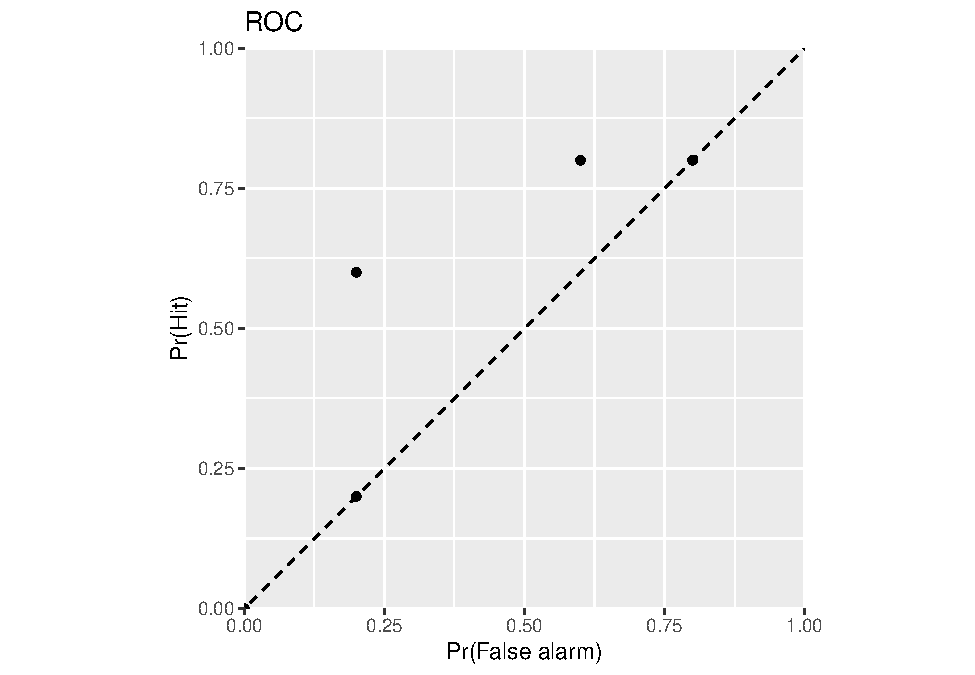
\includegraphics{01-sdt_files/figure-latex/unnamed-chunk-11-1.pdf}

\hypertarget{modeling-strengths}{%
\subsection{Modeling strengths}\label{modeling-strengths}}

We now have a model that instantiates the processes by which strength theory says recognition decisions are made. Pretty neat!

We have \emph{not}, however, modeled the distributions of target and foil strength. Instead, we have just plugged in some numbers. Most SDT theories model these strengths as random variables that are sampled from a distribution.

Another benefit to modeling the strengths is that we can model a situation with a huge number of target/foil trials, far more than would be feasible in any experiment with living creatures. As a result, we can essentially obtain perfect estimates of things like ROC curves by simulating many trials.

\hypertarget{variability-in-initial-strength}{%
\subsubsection{Variability in initial strength}\label{variability-in-initial-strength}}

Let's begin with a simple model in which we assume that all items initially have a strength that is sampled from a normal distribution with mean 0 and standard deviation 1. When an item is studied, its strength is incremented by \emph{exactly} 1.

\begin{Shaded}
\begin{Highlighting}[]
\CommentTok{\# 1. Define one or more decision criteria}
\NormalTok{criteria }\OtherTok{\textless{}{-}} \FunctionTok{c}\NormalTok{(}\SpecialCharTok{{-}}\ConstantTok{Inf}\NormalTok{, }\SpecialCharTok{{-}}\FloatTok{0.5}\NormalTok{, }\DecValTok{0}\NormalTok{, }\FloatTok{0.5}\NormalTok{, }\DecValTok{1}\NormalTok{, }\FloatTok{1.5}\NormalTok{, }\ConstantTok{Inf}\NormalTok{)}

\CommentTok{\# 2. Define the strength of the target (studied) and foil (unstudied) items in memory}
\NormalTok{foil\_strength }\OtherTok{\textless{}{-}} \FunctionTok{rnorm}\NormalTok{(}\AttributeTok{n =} \DecValTok{10000}\NormalTok{, }\AttributeTok{mean =} \DecValTok{0}\NormalTok{, }\AttributeTok{sd =} \DecValTok{1}\NormalTok{)}
\NormalTok{target\_initial\_strength }\OtherTok{\textless{}{-}} \FunctionTok{rnorm}\NormalTok{(}\AttributeTok{n =} \DecValTok{10000}\NormalTok{, }\AttributeTok{mean =} \DecValTok{0}\NormalTok{, }\AttributeTok{sd =} \DecValTok{1}\NormalTok{)}
\NormalTok{study\_strength\_increment }\OtherTok{\textless{}{-}} \DecValTok{1}
\NormalTok{target\_strength }\OtherTok{\textless{}{-}}\NormalTok{ target\_initial\_strength }\SpecialCharTok{+}\NormalTok{ study\_strength\_increment}

\CommentTok{\# 3. Compare the strengths of each test item to the criteria to arrive at a decision}
\NormalTok{foil\_response }\OtherTok{\textless{}{-}} \FunctionTok{cut}\NormalTok{(foil\_strength, }\AttributeTok{breaks=}\NormalTok{criteria, }\AttributeTok{labels=}\ConstantTok{FALSE}\NormalTok{)}
\NormalTok{target\_response }\OtherTok{\textless{}{-}} \FunctionTok{cut}\NormalTok{(target\_strength, }\AttributeTok{breaks=}\NormalTok{criteria, }\AttributeTok{labels=}\ConstantTok{FALSE}\NormalTok{)}

\CommentTok{\# 4. Calculate points on ROC curve}
\NormalTok{roc\_foil }\OtherTok{\textless{}{-}} \DecValTok{1} \SpecialCharTok{{-}} \FunctionTok{ecdf}\NormalTok{(foil\_response)(}\DecValTok{1}\SpecialCharTok{:}\DecValTok{6}\NormalTok{)}
\NormalTok{roc\_target }\OtherTok{\textless{}{-}} \DecValTok{1} \SpecialCharTok{{-}} \FunctionTok{ecdf}\NormalTok{(target\_response)(}\DecValTok{1}\SpecialCharTok{:}\DecValTok{6}\NormalTok{)}

\CommentTok{\# 5. Plot ROC}
\FunctionTok{ggplot}\NormalTok{(}\AttributeTok{mapping=}\FunctionTok{aes}\NormalTok{(}\AttributeTok{x =}\NormalTok{ roc\_foil, }\AttributeTok{y =}\NormalTok{ roc\_target)) }\SpecialCharTok{+}
    \FunctionTok{geom\_point}\NormalTok{() }\SpecialCharTok{+}
    \FunctionTok{geom\_abline}\NormalTok{(}\AttributeTok{intercept =} \DecValTok{0}\NormalTok{, }\AttributeTok{slope =} \DecValTok{1}\NormalTok{, }\AttributeTok{color=}\StringTok{\textquotesingle{}black\textquotesingle{}}\NormalTok{, }\AttributeTok{linetype =} \StringTok{\textquotesingle{}dashed\textquotesingle{}}\NormalTok{) }\SpecialCharTok{+}
    \FunctionTok{labs}\NormalTok{(}\AttributeTok{x =} \StringTok{\textquotesingle{}Pr(False alarm)\textquotesingle{}}\NormalTok{, }\AttributeTok{y =} \StringTok{\textquotesingle{}Pr(Hit)\textquotesingle{}}\NormalTok{, }\AttributeTok{title =} \StringTok{\textquotesingle{}ROC\textquotesingle{}}\NormalTok{) }\SpecialCharTok{+}
    \FunctionTok{coord\_fixed}\NormalTok{(}\AttributeTok{xlim=}\FunctionTok{c}\NormalTok{(}\DecValTok{0}\NormalTok{, }\DecValTok{1}\NormalTok{), }\AttributeTok{ylim=}\FunctionTok{c}\NormalTok{(}\DecValTok{0}\NormalTok{, }\DecValTok{1}\NormalTok{), }\AttributeTok{expand=}\ConstantTok{FALSE}\NormalTok{)}
\end{Highlighting}
\end{Shaded}

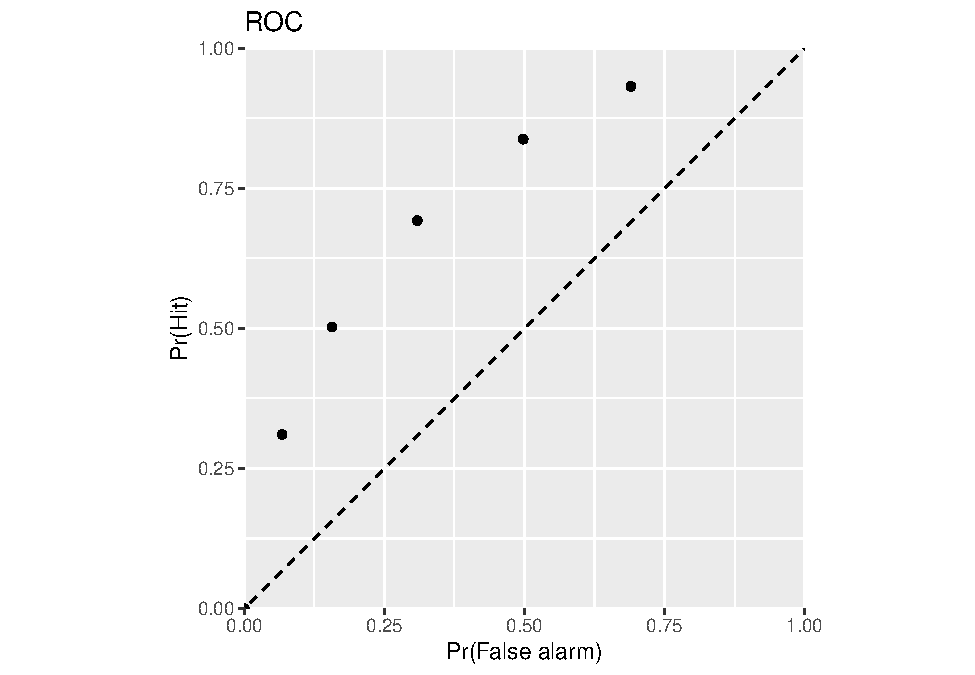
\includegraphics{01-sdt_files/figure-latex/unnamed-chunk-12-1.pdf}

\hypertarget{fine-grained-rocs}{%
\subsubsection{Fine-grained ROC's}\label{fine-grained-rocs}}

Cool! Again, since we're not using a living creature, we can also ask the model to use an absurdly large number of criteria. The value of this is that it gives us a much more fine-grained picture of the ROC. Even though we couldn't get such a picture in real life, if the model is a reasonably good approximation to reality, knowing the detailed model ROC let's us know the kind of shapes we would \emph{expect} to see in an experiment.

\begin{Shaded}
\begin{Highlighting}[]
\CommentTok{\# 1. Define one or more decision criteria}
\NormalTok{num\_criteria }\OtherTok{\textless{}{-}} \DecValTok{100}
\NormalTok{criteria }\OtherTok{\textless{}{-}} \FunctionTok{c}\NormalTok{(}\SpecialCharTok{{-}}\ConstantTok{Inf}\NormalTok{, }\FunctionTok{seq}\NormalTok{(}\SpecialCharTok{{-}}\DecValTok{6}\NormalTok{, }\DecValTok{6}\NormalTok{, }\AttributeTok{length.out =}\NormalTok{ num\_criteria }\SpecialCharTok{{-}} \DecValTok{1}\NormalTok{), }\ConstantTok{Inf}\NormalTok{)}

\CommentTok{\# 2. Define the strength of the target (studied) and foil (unstudied) items in memory}
\NormalTok{foil\_strength }\OtherTok{\textless{}{-}} \FunctionTok{rnorm}\NormalTok{(}\AttributeTok{n =} \DecValTok{10000}\NormalTok{, }\AttributeTok{mean =} \DecValTok{0}\NormalTok{, }\AttributeTok{sd =} \DecValTok{1}\NormalTok{)}
\NormalTok{target\_initial\_strength }\OtherTok{\textless{}{-}} \FunctionTok{rnorm}\NormalTok{(}\AttributeTok{n =} \DecValTok{10000}\NormalTok{, }\AttributeTok{mean =} \DecValTok{0}\NormalTok{, }\AttributeTok{sd =} \DecValTok{1}\NormalTok{)}
\NormalTok{study\_strength\_increment }\OtherTok{\textless{}{-}} \DecValTok{1}
\NormalTok{target\_strength }\OtherTok{\textless{}{-}}\NormalTok{ target\_initial\_strength }\SpecialCharTok{+}\NormalTok{ study\_strength\_increment}

\CommentTok{\# 3. Compare the strengths of each test item to the criteria to arrive at a decision}
\NormalTok{foil\_response }\OtherTok{\textless{}{-}} \FunctionTok{cut}\NormalTok{(foil\_strength, }\AttributeTok{breaks=}\NormalTok{criteria, }\AttributeTok{labels=}\ConstantTok{FALSE}\NormalTok{)}
\NormalTok{target\_response }\OtherTok{\textless{}{-}} \FunctionTok{cut}\NormalTok{(target\_strength, }\AttributeTok{breaks=}\NormalTok{criteria, }\AttributeTok{labels=}\ConstantTok{FALSE}\NormalTok{)}

\CommentTok{\# 4. Calculate points on ROC curve}
\NormalTok{roc\_foil }\OtherTok{\textless{}{-}} \DecValTok{1} \SpecialCharTok{{-}} \FunctionTok{ecdf}\NormalTok{(foil\_response)(}\DecValTok{1}\SpecialCharTok{:}\NormalTok{num\_criteria)}
\NormalTok{roc\_target }\OtherTok{\textless{}{-}} \DecValTok{1} \SpecialCharTok{{-}} \FunctionTok{ecdf}\NormalTok{(target\_response)(}\DecValTok{1}\SpecialCharTok{:}\NormalTok{num\_criteria)}

\CommentTok{\# 5. Plot ROC}
\FunctionTok{ggplot}\NormalTok{(}\AttributeTok{mapping=}\FunctionTok{aes}\NormalTok{(}\AttributeTok{x =}\NormalTok{ roc\_foil, }\AttributeTok{y =}\NormalTok{ roc\_target)) }\SpecialCharTok{+}
    \FunctionTok{geom\_line}\NormalTok{() }\SpecialCharTok{+}
    \FunctionTok{geom\_abline}\NormalTok{(}\AttributeTok{intercept =} \DecValTok{0}\NormalTok{, }\AttributeTok{slope =} \DecValTok{1}\NormalTok{, }\AttributeTok{color=}\StringTok{\textquotesingle{}black\textquotesingle{}}\NormalTok{, }\AttributeTok{linetype =} \StringTok{\textquotesingle{}dashed\textquotesingle{}}\NormalTok{) }\SpecialCharTok{+}
    \FunctionTok{labs}\NormalTok{(}\AttributeTok{x =} \StringTok{\textquotesingle{}Pr(False alarm)\textquotesingle{}}\NormalTok{, }\AttributeTok{y =} \StringTok{\textquotesingle{}Pr(Hit)\textquotesingle{}}\NormalTok{, }\AttributeTok{title =} \StringTok{\textquotesingle{}ROC\textquotesingle{}}\NormalTok{) }\SpecialCharTok{+}
    \FunctionTok{coord\_fixed}\NormalTok{(}\AttributeTok{xlim=}\FunctionTok{c}\NormalTok{(}\DecValTok{0}\NormalTok{, }\DecValTok{1}\NormalTok{), }\AttributeTok{ylim=}\FunctionTok{c}\NormalTok{(}\DecValTok{0}\NormalTok{, }\DecValTok{1}\NormalTok{), }\AttributeTok{expand=}\ConstantTok{FALSE}\NormalTok{)}
\end{Highlighting}
\end{Shaded}

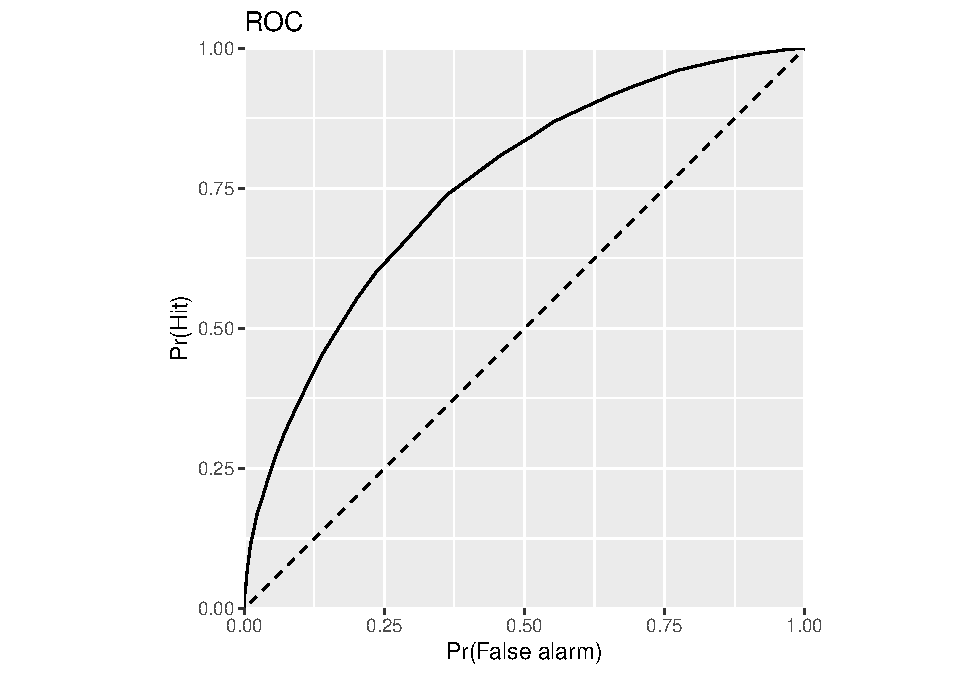
\includegraphics{01-sdt_files/figure-latex/unnamed-chunk-13-1.pdf}

\hypertarget{variability-in-study-strength-increments}{%
\subsubsection{Variability in study strength increments}\label{variability-in-study-strength-increments}}

Finally, let's introduce variability in the increment in strength that results from studying an item. Again, maybe we can imagine this strength increment comes from a normal distribution (this is the assumption of the unequal-variance SDT model). In that case, we can define its mean and standard deviation.

\begin{Shaded}
\begin{Highlighting}[]
\CommentTok{\# 1. Define one or more decision criteria}
\NormalTok{num\_criteria }\OtherTok{\textless{}{-}} \DecValTok{100}
\NormalTok{criteria }\OtherTok{\textless{}{-}} \FunctionTok{c}\NormalTok{(}\SpecialCharTok{{-}}\ConstantTok{Inf}\NormalTok{, }\FunctionTok{seq}\NormalTok{(}\SpecialCharTok{{-}}\DecValTok{6}\NormalTok{, }\DecValTok{6}\NormalTok{, }\AttributeTok{length.out =}\NormalTok{ num\_criteria }\SpecialCharTok{{-}} \DecValTok{1}\NormalTok{), }\ConstantTok{Inf}\NormalTok{)}

\CommentTok{\# 2. Define the strength of the target (studied) and foil (unstudied) items in memory}
\NormalTok{foil\_strength }\OtherTok{\textless{}{-}} \FunctionTok{rnorm}\NormalTok{(}\AttributeTok{n =} \DecValTok{10000}\NormalTok{, }\AttributeTok{mean =} \DecValTok{0}\NormalTok{, }\AttributeTok{sd =} \DecValTok{1}\NormalTok{)}
\NormalTok{target\_initial\_strength }\OtherTok{\textless{}{-}} \FunctionTok{rnorm}\NormalTok{(}\AttributeTok{n =} \DecValTok{10000}\NormalTok{, }\AttributeTok{mean =} \DecValTok{0}\NormalTok{, }\AttributeTok{sd =} \DecValTok{1}\NormalTok{)}
\NormalTok{study\_strength\_increment }\OtherTok{\textless{}{-}} \FunctionTok{rnorm}\NormalTok{(}\AttributeTok{n =} \DecValTok{10000}\NormalTok{, }\AttributeTok{mean =} \DecValTok{1}\NormalTok{, }\AttributeTok{sd =} \DecValTok{1}\NormalTok{)}
\NormalTok{target\_strength }\OtherTok{\textless{}{-}}\NormalTok{ target\_initial\_strength }\SpecialCharTok{+}\NormalTok{ study\_strength\_increment}

\CommentTok{\# 3. Compare the strengths of each test item to the criteria to arrive at a decision}
\NormalTok{foil\_response }\OtherTok{\textless{}{-}} \FunctionTok{cut}\NormalTok{(foil\_strength, }\AttributeTok{breaks=}\NormalTok{criteria, }\AttributeTok{labels=}\ConstantTok{FALSE}\NormalTok{)}
\NormalTok{target\_response }\OtherTok{\textless{}{-}} \FunctionTok{cut}\NormalTok{(target\_strength, }\AttributeTok{breaks=}\NormalTok{criteria, }\AttributeTok{labels=}\ConstantTok{FALSE}\NormalTok{)}

\CommentTok{\# 4. Calculate points on ROC curve}
\NormalTok{roc\_foil }\OtherTok{\textless{}{-}} \DecValTok{1} \SpecialCharTok{{-}} \FunctionTok{ecdf}\NormalTok{(foil\_response)(}\DecValTok{1}\SpecialCharTok{:}\NormalTok{num\_criteria)}
\NormalTok{roc\_target }\OtherTok{\textless{}{-}} \DecValTok{1} \SpecialCharTok{{-}} \FunctionTok{ecdf}\NormalTok{(target\_response)(}\DecValTok{1}\SpecialCharTok{:}\NormalTok{num\_criteria)}

\CommentTok{\# 5. Plot ROC}
\FunctionTok{ggplot}\NormalTok{(}\AttributeTok{mapping=}\FunctionTok{aes}\NormalTok{(}\AttributeTok{x =}\NormalTok{ roc\_foil, }\AttributeTok{y =}\NormalTok{ roc\_target)) }\SpecialCharTok{+}
    \FunctionTok{geom\_line}\NormalTok{() }\SpecialCharTok{+}
    \FunctionTok{geom\_abline}\NormalTok{(}\AttributeTok{intercept =} \DecValTok{0}\NormalTok{, }\AttributeTok{slope =} \DecValTok{1}\NormalTok{, }\AttributeTok{color=}\StringTok{\textquotesingle{}black\textquotesingle{}}\NormalTok{, }\AttributeTok{linetype =} \StringTok{\textquotesingle{}dashed\textquotesingle{}}\NormalTok{) }\SpecialCharTok{+}
    \FunctionTok{labs}\NormalTok{(}\AttributeTok{x =} \StringTok{\textquotesingle{}Pr(False alarm)\textquotesingle{}}\NormalTok{, }\AttributeTok{y =} \StringTok{\textquotesingle{}Pr(Hit)\textquotesingle{}}\NormalTok{, }\AttributeTok{title =} \StringTok{\textquotesingle{}ROC\textquotesingle{}}\NormalTok{) }\SpecialCharTok{+}
    \FunctionTok{coord\_fixed}\NormalTok{(}\AttributeTok{xlim=}\FunctionTok{c}\NormalTok{(}\DecValTok{0}\NormalTok{, }\DecValTok{1}\NormalTok{), }\AttributeTok{ylim=}\FunctionTok{c}\NormalTok{(}\DecValTok{0}\NormalTok{, }\DecValTok{1}\NormalTok{), }\AttributeTok{expand=}\ConstantTok{FALSE}\NormalTok{)}
\end{Highlighting}
\end{Shaded}

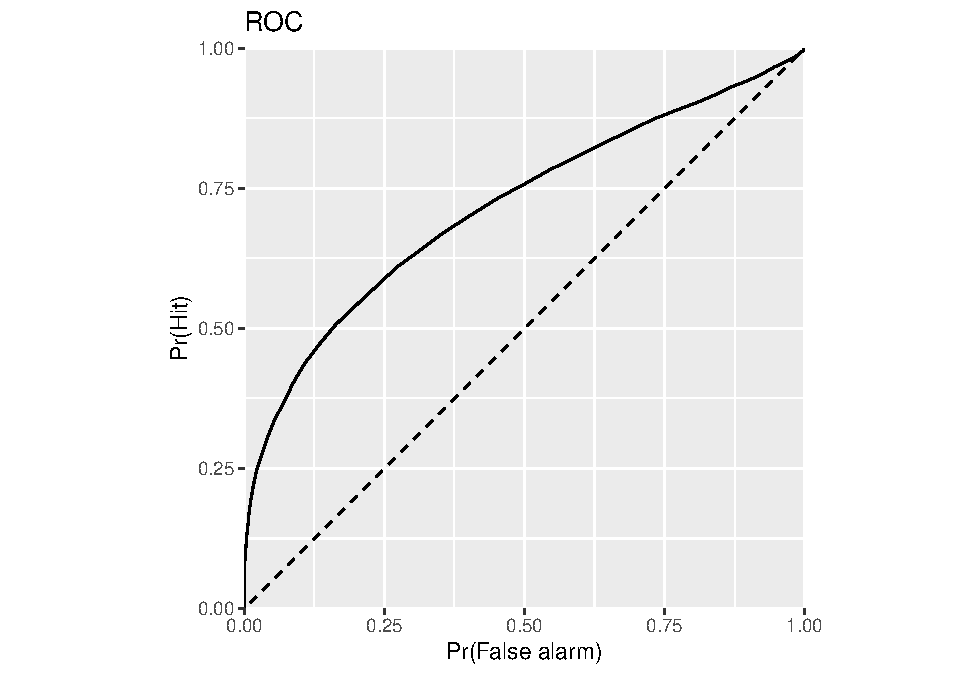
\includegraphics{01-sdt_files/figure-latex/unnamed-chunk-14-1.pdf}

\hypertarget{going-off-trail}{%
\section{Going off-trail}\label{going-off-trail}}

Following the trail this far has gotten us to a reasonably complete model of recognition by signal detection, according to strength theory. Now it's your turn to go off-trail and explore on your own!

\begin{enumerate}
\def\labelenumi{\arabic{enumi}.}
\tightlist
\item
  If study strength increments are normally distributed, this means it is possible for them to be \emph{negative}, that is, for studying an item to actually decrease its strength from its initial level. Could this be plausible under some circumstances? If it is plausible, what does this say about how we should interpret what ``strength'' means in this context?
\item
  Try swapping out the normally-distributed strength increment for one that is \emph{exponentially} distributed. In R, you can draw random samples from an exponential distribution with the \texttt{rexp} function (check out the help pages to see what parameters the function takes). How close can you get the resulting ROC to looking linear across most of its range? What does this say about the kinds of conclusions we can draw based on the shape of ROC's? Are there reasons why the exponential distribution might be a better or worse model for study strength increments?
\item
  Pick an alternative recognition model (e.g., a threshold model or a hybrid model or one of your own ideas) and implement it by modifying the code we built on trail. What choices did you make about how to implement the model you chose and why? Did you stick with the same basic structure as the model we built above, or did you modify it at all? Were you able to find any unique or striking---but still plausible---predictions from your chosen model?
\end{enumerate}

  \bibliography{book.bib,packages.bib}

\end{document}
